\documentclass[11pt,a4paper]{article}
\usepackage[utf8]{inputenc}
\usepackage[T1]{fontenc}
\usepackage{array}
\usepackage{amsmath}
\usepackage{amsfonts}
\usepackage{siunitx}
\usepackage[section]{placeins}
\usepackage{amssymb}
\usepackage{makeidx}
\usepackage{sidecap}
\usepackage{fvextra}
\usepackage{multicol}
\usepackage{listings}
\usepackage{appendix}
\usepackage{comment}
\usepackage{nicematrix}
\usepackage{multirow}
\usepackage{braket}
\usepackage{graphicx}
\usepackage{relsize}
\usepackage{fancyhdr}
\usepackage{cprotect}
\usepackage{color} 
\usepackage{hyperref}
\hypersetup{
	colorlinks=true, 
	linktoc=all, 
	linkcolor=blue,
	urlcolor=blue
}
\usepackage[left=2cm,right=2cm,top=1.5cm,bottom=2cm]{geometry}
\usepackage{titling}
\usepackage{etoolbox}
\flushbottom
\title{Statistical Analysis of Experimental Data\\
	\vspace{0.2cm}
	\large{Homework 07}}
\vspace{-0.2cm}
\author{Igor Di Tota}
\date{\small \url{https://github.com/igordt/SAED_homeworks/tree/main}}


\begin{document}
	
	\maketitle
	
	\section*{Introduction}

	This homework concerns the least-squares method: \textit{download the set of data from the lecture home page (text file with three columns: $x_i$, $y_i$, $\sigma_{y_i}$). Use linear regression method to fit polynomial dependence to the data. Calculate p-value for the 3rd and 4th order polynomial fit. Point to the order of polynomial, which is adequate for the description of the data and give arguments for your choice.}

	The data are described with a polynomial
	\begin{equation}
		\mu(x; \mathbf{a}) = \sum_{k=0}^{M} a_k\, x^k ,
	\end{equation}
	where $M$ is the order of the polynomial and $\mathbf{a} = (a_0, \dots, a_M)$ are the $M+1$ free parameters.
	Since the model is linear in the parameters, the least-squares method gives the best estimates of $\mathbf{a}$ and their covariance matrix by solving a system of linear equations.
	Assuming Gaussian measurement uncertainties and a correct model, the value of $\chi^2$ at the minimum follows a $\chi^2$ distribution with $N_{df} = N - (M+1)$ degrees of freedom, so it can be used to test whether the polynomial of order $M$ is consistent with the data.

	\section*{Data}

	The data set consists of $N = 24$ points, shown in Figure~\ref{fig:data}.
	Each value $y_i$ is given with its uncertainty $\sigma_i$, which is not constant but increases with $x$, from about $0.021$ to $0.050$.
	The measurements therefore have different weights in the fit, and each term of the $\chi^2$ must be divided by its own $\sigma_i^2$.
	The dependence of $y$ on $x$ is clearly not linear. No model for this dependence is given, so polynomials of increasing order are tested.

	\begin{figure}[htbp]
		\centering
		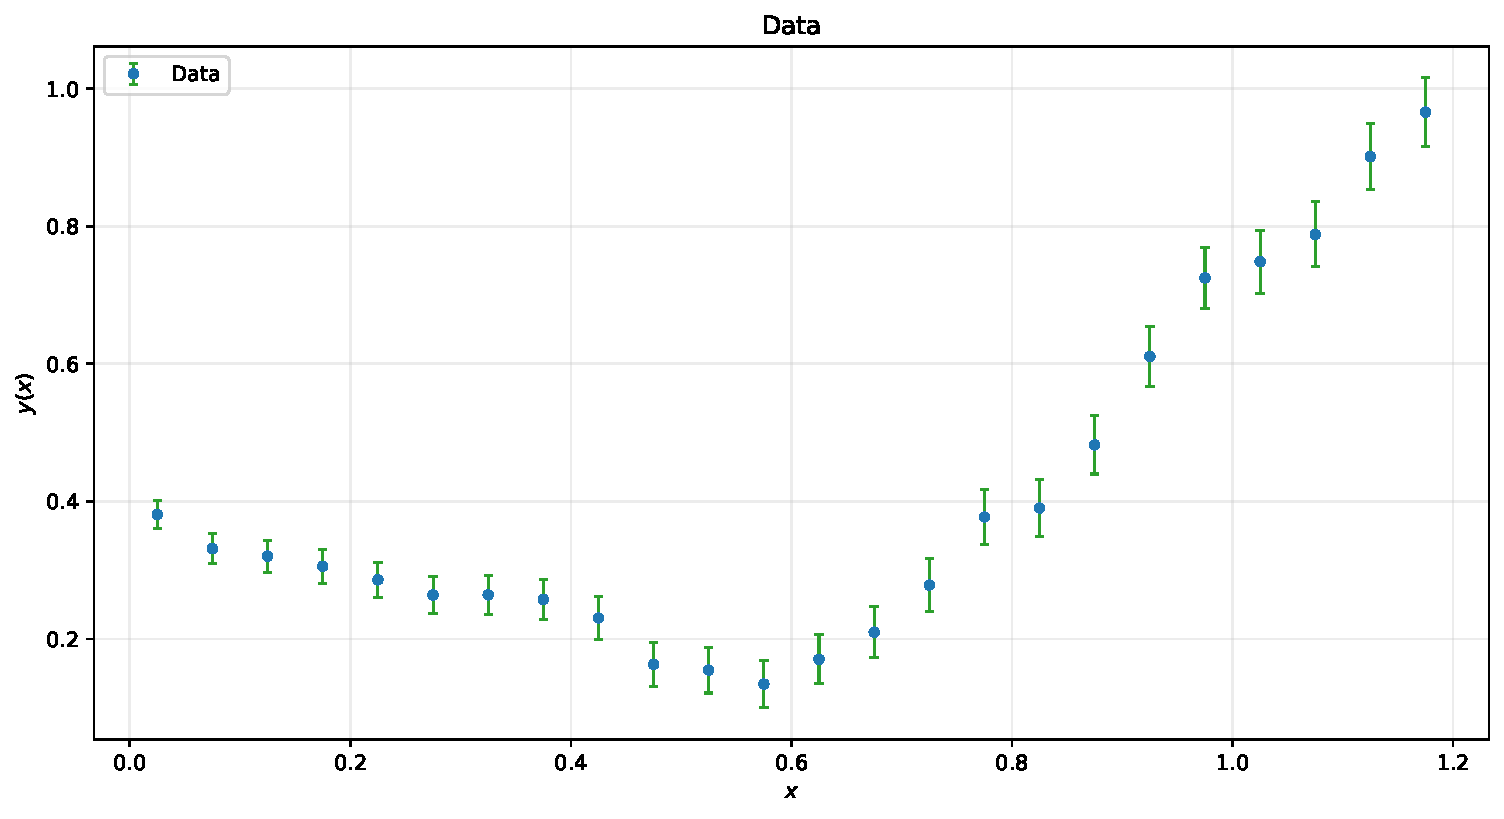
\includegraphics[width=\linewidth]{images/data.pdf}
		\caption{Data set: measured values $y_i$ with their uncertainties $\sigma_i$.}
		\label{fig:data}
	\end{figure}

	\section*{Linear regression}

	The model is linear in the parameters, $\mu(x; \mathbf{a}) = \sum_{k=0}^{M} a_k f_k(x)$ with $f_k(x) = x^k$.
	The best estimates of $\mathbf{a}$ correspond to the minimum of
	\begin{equation}
		\chi^2(\mathbf{a}) = \sum_{i=1}^{N} \frac{\left(y_i - \sum_{k} a_k f_k(x_i)\right)^2}{\sigma_i^2} ,
	\end{equation}
	which, for Gaussian uncertainties, is equivalent to the maximum of the log-likelihood function $\ell = \ln L$, since $\chi^2 = -2\ell$ (up to a constant factor).

	Setting $\partial\chi^2/\partial a_l = 0$ for $l = 0, \dots, M$ gives a system of $M+1$ linear equations
	\begin{equation}
		\sum_{k=0}^{M} \left( \sum_{i=1}^{N} \frac{f_l(x_i)\, f_k(x_i)}{\sigma_i^2} \right) a_k = \sum_{i=1}^{N} \frac{f_l(x_i)\, y_i}{\sigma_i^2} ,
	\end{equation}
	which can be written in matrix form as $\mathbb{A}\cdot\mathbf{a} = \mathbf{b}$, with
	\begin{equation}
		\mathbb{A}_{lk} = \sum_{i=1}^{N} \frac{x_i^{\,l+k}}{\sigma_i^2} ,
		\qquad
		b_l = \sum_{i=1}^{N} \frac{x_i^{\,l}\, y_i}{\sigma_i^2} ,
		\qquad
		\mathbf{a} = \mathbb{A}^{-1} \cdot \mathbf{b} .
	\end{equation}

	The first derivatives of the $\chi^2$ are
	\begin{equation}
		\frac{\partial\chi^2}{\partial a_l} = -2 \sum_{i=1}^{N} \frac{f_l(x_i)}{\sigma_i^2} \left( y_i - \sum_{k=0}^{M} a_k f_k(x_i) \right) ,
	\end{equation}
	and differentiating once more with respect to $a_k$,
	\begin{equation}
		\frac{\partial^2\chi^2}{\partial a_l\, \partial a_k} = 2 \sum_{i=1}^{N} \frac{f_l(x_i)\, f_k(x_i)}{\sigma_i^2} = 2\,\mathbb{A}_{lk} .
	\end{equation}
	The second derivatives do not depend on $\mathbf{a}$: the $\chi^2$ is exactly a quadratic function of the parameters, so the parabolic approximation used in the maximum likelihood method to derive the covariance matrix is exact in this case, and
	\begin{equation}
		\mathbb{C}_{\mathbf{a}} = \left(-\frac{\partial^2 \ell}{\partial a_l\, \partial a_k}\right)^{-1} = \left(\frac{1}{2}\frac{\partial^2\chi^2}{\partial a_l\, \partial a_k}\right)^{-1} = \mathbb{A}^{-1} .
	\end{equation}

	The quality of the fit is described by the value $\chi^2_{min}$ at the minimum which, if the model is correct, follows a $\chi^2$ distribution with $N_{df} = N - (M+1)$ degrees of freedom.
	The p-value is the probability of obtaining a value equal to or larger than the observed one, if the model is correct:
	\begin{equation}
		p = \int_{\chi^2_{min}}^{+\infty} f_{\chi^2}(t; N_{df})\, dt = 1 - P(\chi^2_{min}; N_{df}),
	\end{equation}
	where $f_{\chi^2}$ is the $\chi^2$ probability density and $P$ its cumulative distribution function.

	\subsection*{Implementation}

	For each order $M$, the matrix $\mathbb{A}$ and the vector $\mathbf{b}$ are built following directly their definitions.
	The system $\mathbb{A}\cdot\mathbf{a} = \mathbf{b}$ is solved with \texttt{np.linalg.solve}.
	The p-value is computed as $1 - P(\chi^2_{min}; N_{df})$ with the cumulative distribution function \texttt{stats.chi2.cdf}; for very small p-values (below about $10^{-16}$) the result is rounded to zero, since $P(\chi^2_{min}; N_{df})$ cannot be distinguished from 1.

	\section*{Fit results}

	The polynomials of order $M = 0, \dots, 8$ are fitted to the data; the results are reported in Table~\ref{tab:fits}.
	The column $\Delta\chi^2$ is the decrease of $\chi^2_{min}$ with respect to the polynomial of order $M-1$, obtained by adding one parameter to the model.

	\begin{table}[htbp]
		\centering
		\begin{tabular}{ccrrrcr}
			\hline
			$M$ & $N_{par}$ & $\chi^2_{min}$ & $N_{df}$ & $\chi^2_{min}/N_{df}$ & p-value & $\Delta\chi^2$ \\
			\hline
			0 & 1 & 767.52 & 23 & 33.37 & $< 10^{-16}$ & -- \\
			1 & 2 & 538.57 & 22 & 24.48 & $< 10^{-16}$ & 228.96 \\
			2 & 3 & 50.20 & 21 & 2.39 & $3.4 \cdot 10^{-4}$ & 488.36 \\
			3 & 4 & 39.52 & 20 & 1.98 & $5.7 \cdot 10^{-3}$ & 10.68 \\
			4 & 5 & 20.39 & 19 & 1.07 & $0.37$ & 19.14 \\
			5 & 6 & 13.37 & 18 & 0.74 & $0.77$ & 7.01 \\
			6 & 7 & 7.08 & 17 & 0.42 & $0.982$ & 6.29 \\
			7 & 8 & 6.47 & 16 & 0.40 & $0.982$ & 0.61 \\
			8 & 9 & 6.20 & 15 & 0.41 & $0.976$ & 0.28 \\
			\hline
		\end{tabular}
		\caption{Results of the fits of polynomials of order $M$: number of parameters, $\chi^2$ at the minimum, number of degrees of freedom, p-value and decrease of the $\chi^2$ with respect to the order $M-1$.}
		\label{tab:fits}
	\end{table}

	The polynomials of order $M = 2, \dots, 6$ are compared with the data in Figure~\ref{fig:fits}; the orders $M = 0$ and $M = 1$ are not shown, since they clearly cannot describe the data.

	\begin{figure}[htbp]
		\centering
		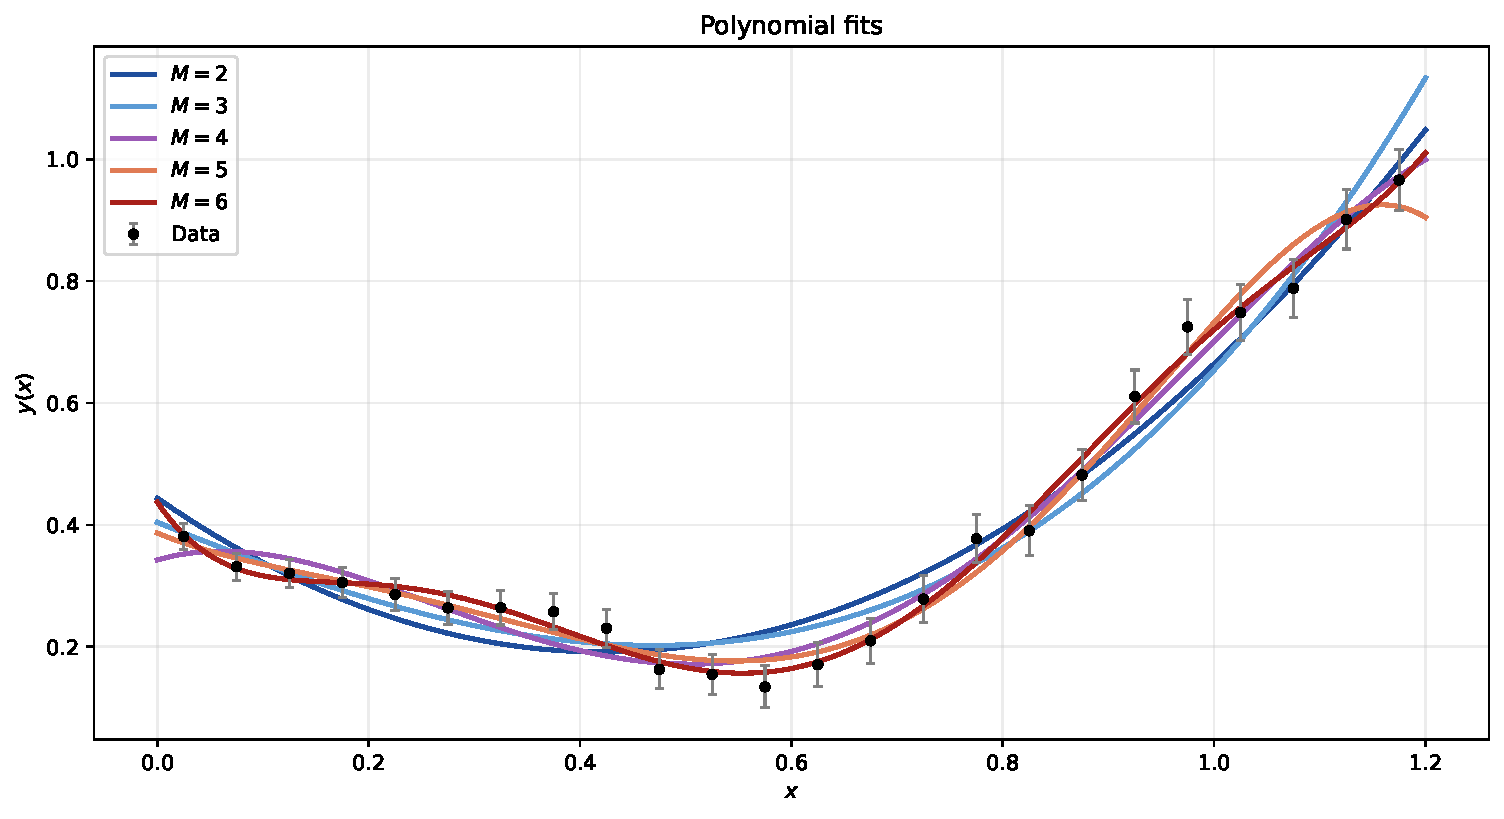
\includegraphics[width=\linewidth]{images/fits.pdf}
		\caption{Polynomial fits of order $M = 2, \dots, 6$ compared with the data.}
		\label{fig:fits}
	\end{figure}

	\subsection*{High order polynomials}

	The polynomials of order $M = 6, 7, 8$ are compared in Figure~\ref{fig:high_order}.
	In the range of the data the three curves are practically indistinguishable, consistently with the very small decrease of $\chi^2_{min}$ ($\Delta\chi^2 < 1$) obtained by adding the corresponding parameters.
	The curves differ only at the edges of the interval, shown in the two zoomed panels: at the measurement points the differences between them are at most about half of the uncertainty $\sigma_i$, and they become larger only outside the range of the data ($x < 0.025$ and $x > 1.175$), where the polynomials are not constrained by any measurement.

	\begin{figure}[htbp]
		\centering
		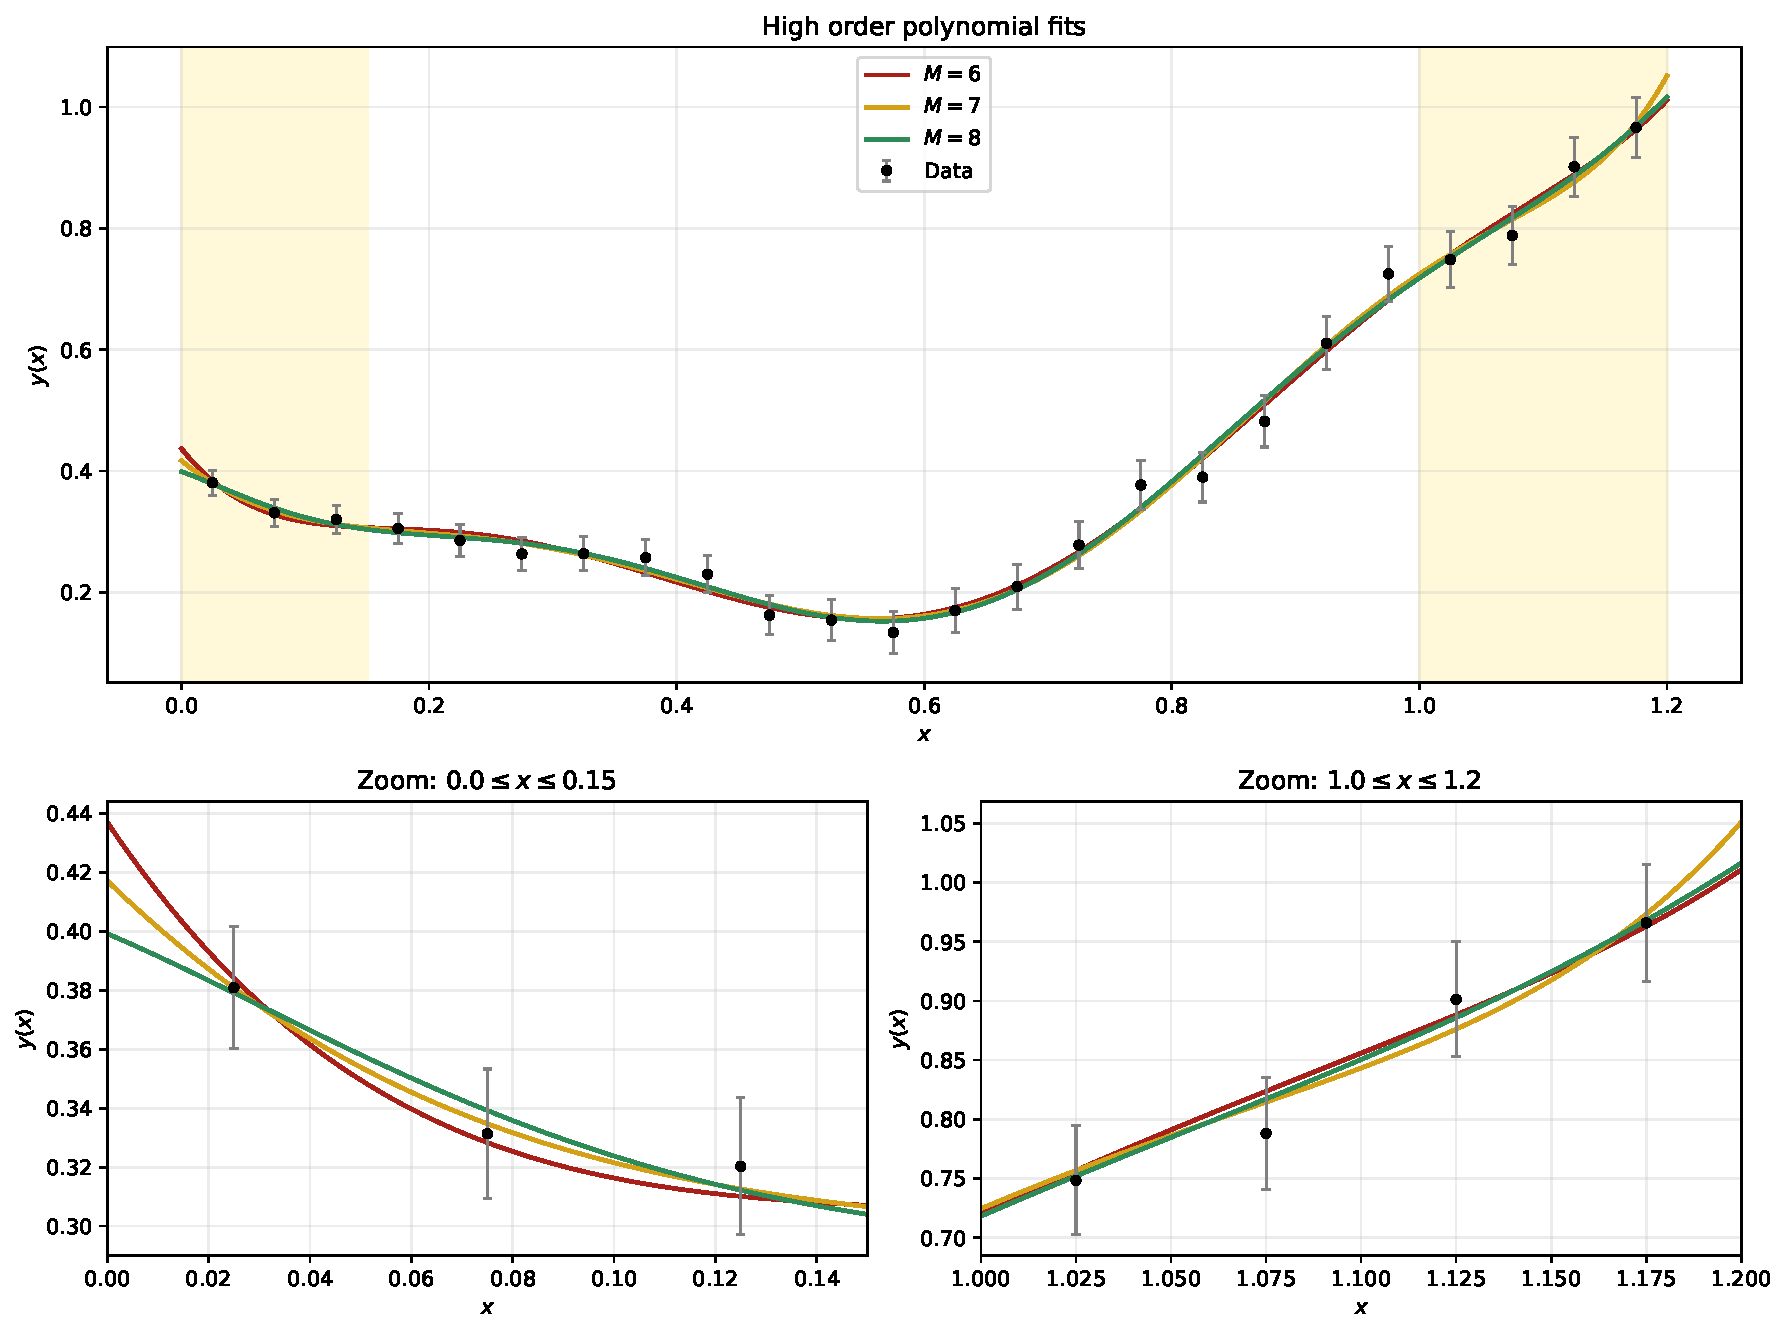
\includegraphics[width=\linewidth]{images/fits_high_order.pdf}
		\caption{Top: polynomial fits of order $M = 6, 7, 8$; the shaded regions are shown enlarged in the bottom panels. Bottom: zoom on the two edges of the interval.}
		\label{fig:high_order}
	\end{figure}

	\section*{Normalized residuals}

	The agreement between the data and each fit is studied with the normalized residuals
	\begin{equation}
		r_i = \frac{y_i - \mu(x_i; \mathbf{a})}{\sigma_i} ,
	\end{equation}
	whose sum of squares is $\chi^2_{min}$.
	If the model is correct, the residuals fluctuate randomly around zero, with about 68\% of them within $\pm 1$ and about 95\% within $\pm 2$.
	If the order of the polynomial is too low, the residuals deviate systematically from zero in some regions of $x$.
	If the order is too high, the polynomial starts to follow the fluctuations of the data and the residuals become smaller than expected.

	The residuals for the orders $M = 3, 4, 5, 6$ are shown in Figure~\ref{fig:residuals}; Table~\ref{tab:residuals} reports the largest residual in absolute value and the fractions of residuals within $\pm 1$ and $\pm 2$.

	\begin{table}[htbp]
		\centering
		\begin{tabular}{cccc}
			\hline
			$M$ & $\max_i |r_i|$ & fraction $|r_i| < 1$ & fraction $|r_i| < 2$ \\
			\hline
			3 & 2.61 & 0.54 & 0.92 \\
			4 & 1.79 & 0.67 & 1.00 \\
			5 & 1.53 & 0.83 & 1.00 \\
			6 & 0.97 & 1.00 & 1.00 \\
			\hline
		\end{tabular}
		\caption{Normalized residuals: largest value and fractions within $\pm 1$ and $\pm 2$, to be compared with the expected values of about 0.68 and 0.95.}
		\label{tab:residuals}
	\end{table}

	\begin{figure}[htbp]
		\centering
		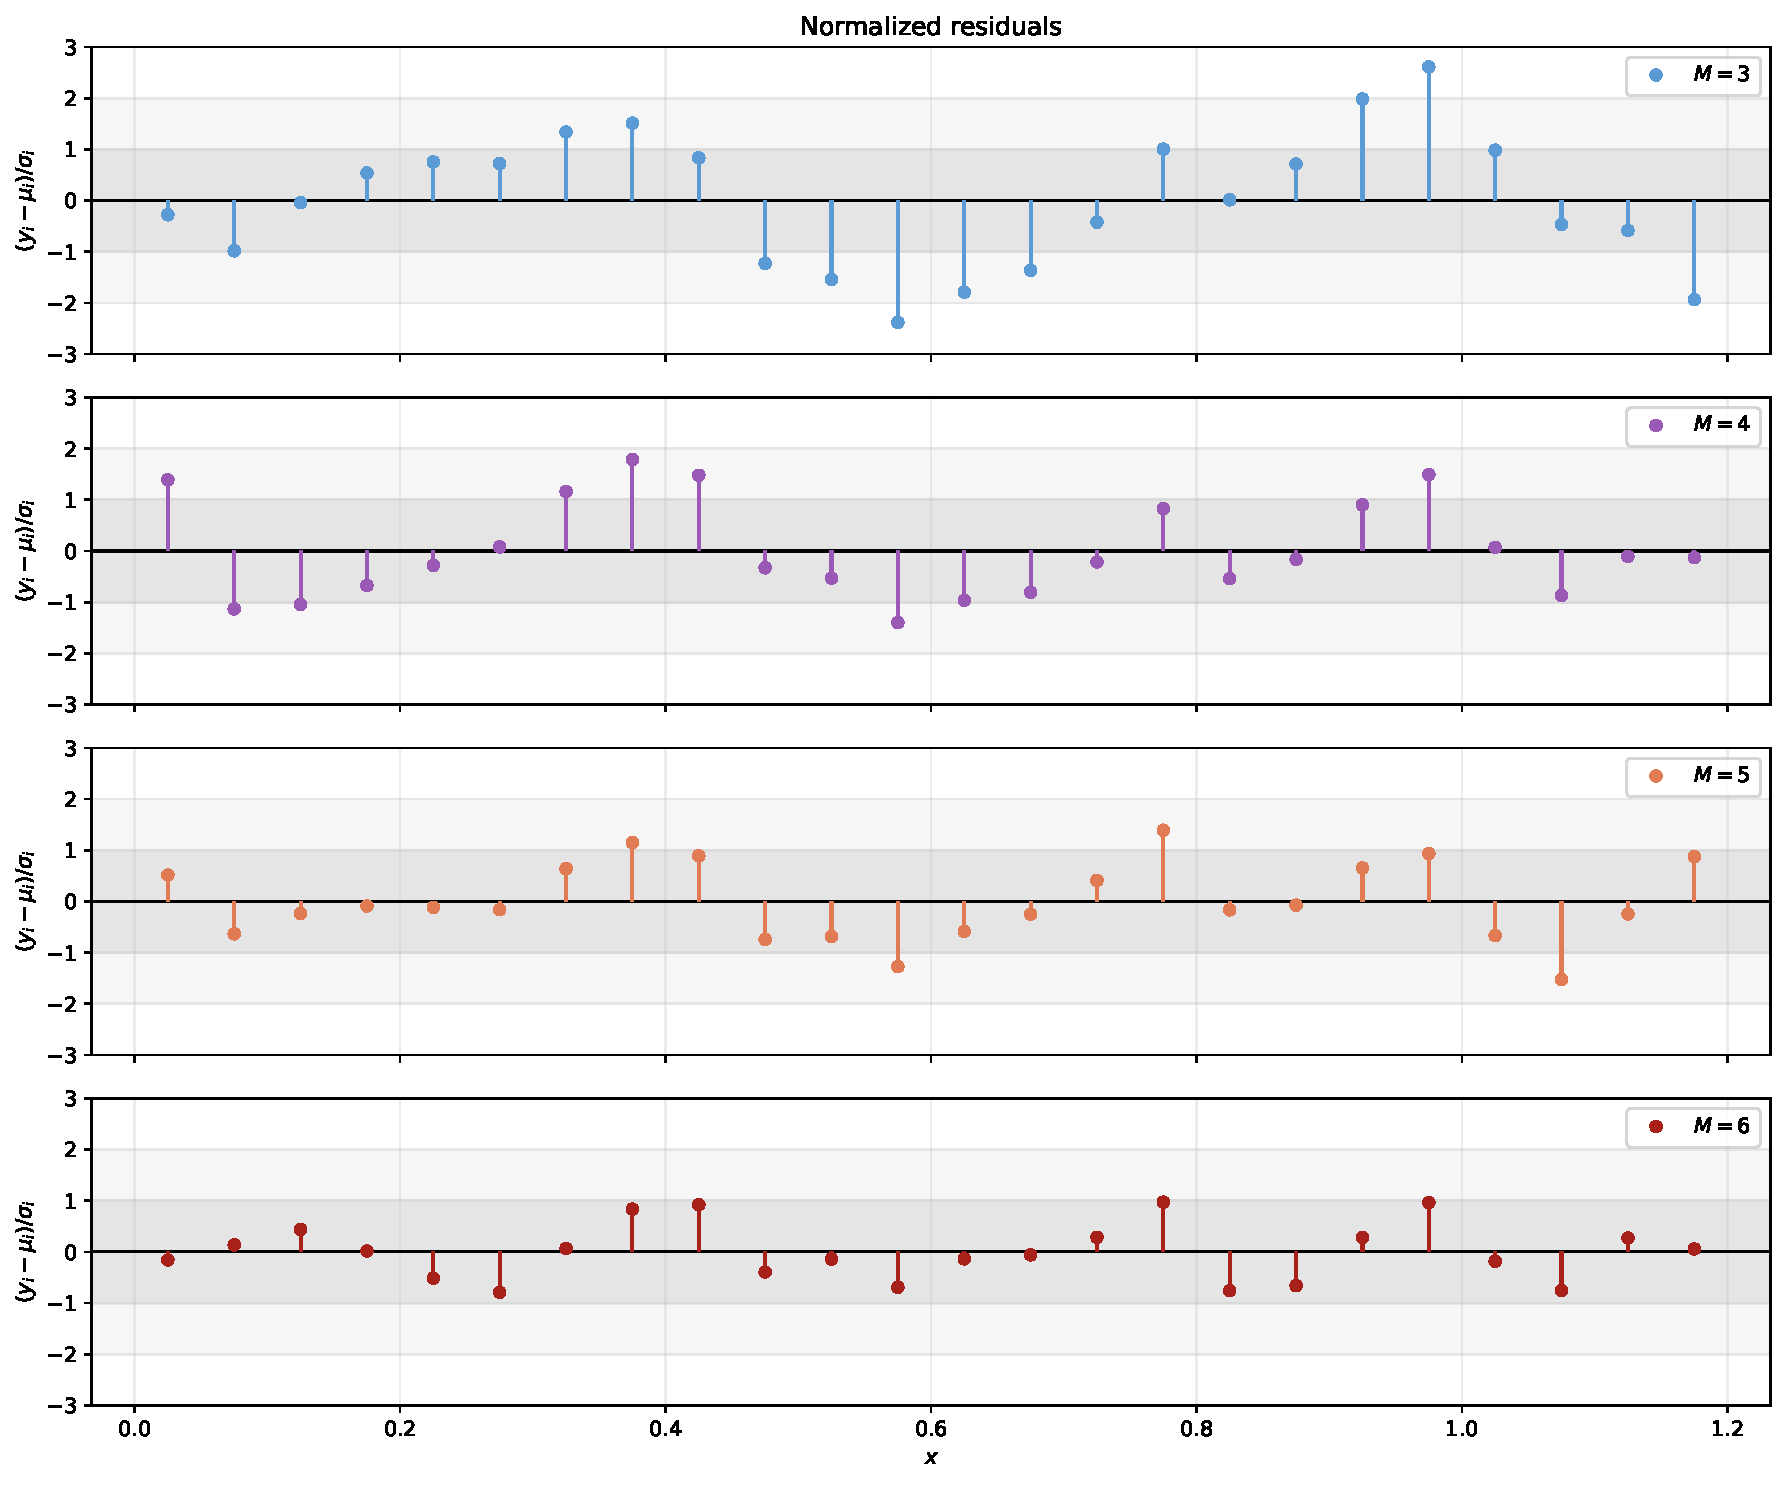
\includegraphics[width=0.8\linewidth]{images/residuals.pdf}
		\caption{Normalized residuals for the polynomials of order $M = 3, 4, 5, 6$. The shaded bands correspond to $|r_i| < 1$ and $|r_i| < 2$.}
		\label{fig:residuals}
	\end{figure}

	\section*{Parameters and correlations}

	The uncertainties of the parameters are given by the diagonal elements of the covariance matrix, $\sigma(a_k) = \sqrt{(\mathbb{C}_{\mathbf{a}})_{kk}}$, and the correlation coefficients by
	\begin{equation}
		\rho_{lk} = \frac{(\mathbb{C}_{\mathbf{a}})_{lk}}{\sigma(a_l)\, \sigma(a_k)} .
	\end{equation}

	When the order of the polynomial is increased from $M-1$ to $M$, the new parameter $a_M$ is added to the model.
	If the polynomial of order $M-1$ already describes the data, the additional parameter is not needed and its fitted value is expected to be consistent with zero.
	This is quantified by the significance of the last coefficient, i.e. its distance from zero in units of its uncertainty, $\hat a_M / \sigma(a_M)$: values of $|\hat a_M| / \sigma(a_M)$ of order 1 are expected if the parameter is not needed, while values of 3 or more indicate that $a_M$ is significantly different from zero.

	For a model linear in the parameters, the significance of $a_M$ is directly related to the decrease of the $\chi^2$ obtained by adding it to the model.
	Since the $\chi^2$ is exactly quadratic in the parameters, the $\chi^2$ minimized with respect to all the other parameters is, as a function of $a_M$ alone, a parabola with its minimum at $\hat a_M$ and increasing by 1 at $\hat a_M \pm \sigma(a_M)$:
	\begin{equation}
		\chi^2(a_M) = \chi^2_{min}(M) + \left(\frac{a_M - \hat a_M}{\sigma(a_M)}\right)^2 .
	\end{equation}
	The polynomial of order $M-1$ corresponds to $a_M = 0$, therefore
	\begin{equation}
		\Delta\chi^2 = \chi^2_{min}(M-1) - \chi^2_{min}(M) = \left(\frac{\hat a_M}{\sigma(a_M)}\right)^2 ,
	\end{equation}
	so a significant decrease of the $\chi^2$ corresponds to a value of $a_M$ significantly different from zero.
	Since $\hat{\mathbf{a}}$ is a linear function of the Gaussian measurements $y_i$, the estimate $\hat a_M$ is Gaussian with standard deviation $\sigma(a_M)$.
	If the parameter is not needed (true value $a_M = 0$), $\hat a_M / \sigma(a_M)$ follows a standard Gaussian distribution and $\Delta\chi^2$, its square, follows a $\chi^2$ distribution with one degree of freedom, with mean value 1: values $\Delta\chi^2 < 3.84$ are expected with 95\% probability, and values $\Delta\chi^2 > 9$ only with 0.3\% probability.
	The p-value of $\Delta\chi^2$, computed with the $\chi^2$ distribution for one degree of freedom, gives the probability of a decrease equal to or larger than the observed one if the additional parameter is not needed.

	Other indications that the polynomial has too many parameters are a strong increase of the values and of the uncertainties of the parameters, since the polynomial becomes a sum of large contributions cancelling each other, and correlations between the parameters approaching $\pm 1$.

	These quantities are reported in Table~\ref{tab:parameters}, and the correlation matrices for the orders $M = 3, 4, 5$ are shown in Figure~\ref{fig:correlations}.

	\begin{table}[htbp]
		\centering
		\begin{tabular}{crrrrcc}
			\hline
			$M$ & $\hat a_M$ & $\sigma(a_M)$ & $\hat a_M/\sigma(a_M)$ & $\Delta\chi^2$ & $p(\Delta\chi^2)$ & $\max_{l \neq k} |\rho_{lk}|$ \\
			\hline
			1 & 0.300 & 0.020 & 15.13 & 228.96 & $< 10^{-16}$ & 0.790 \\
			2 & 1.416 & 0.064 & 22.10 & 488.36 & $< 10^{-16}$ & 0.960 \\
			3 & 0.694 & 0.212 & 3.27 & 10.68 & $1.1 \cdot 10^{-3}$ & 0.984 \\
			4 & $-3.121$ & 0.713 & $-4.37$ & 19.14 & $1.2 \cdot 10^{-5}$ & 0.992 \\
			5 & $-6.414$ & 2.422 & $-2.65$ & 7.01 & $8.1 \cdot 10^{-3}$ & 0.995 \\
			6 & 20.877 & 8.321 & 2.51 & 6.29 & $1.2 \cdot 10^{-2}$ & 0.997 \\
			7 & 22.589 & 28.969 & 0.78 & 0.61 & 0.44 & 0.998 \\
			8 & $-53.882$ & 102.394 & $-0.53$ & 0.28 & 0.60 & 0.998 \\
			\hline
		\end{tabular}
		\caption{Last coefficient $\hat a_M$ of the polynomial of order $M$, its uncertainty and significance, decrease of the $\chi^2$ with respect to the order $M-1$ with its p-value for a $\chi^2$ distribution with one degree of freedom, and largest correlation between two different parameters.}
		\label{tab:parameters}
	\end{table}

	\begin{figure}[htbp]
		\centering
		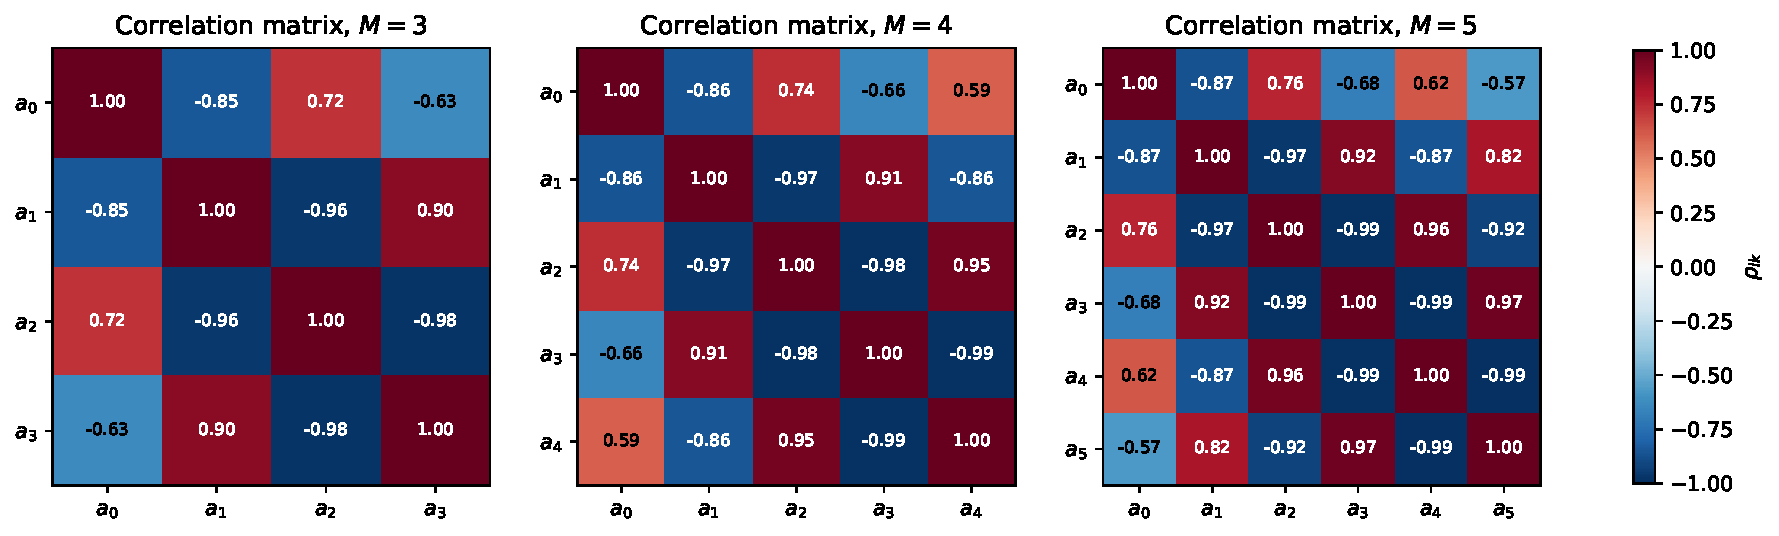
\includegraphics[width=\linewidth]{images/correlations.pdf}
		\caption{Correlation matrices $\rho_{lk}$ of the parameters of the polynomials of order $M = 3, 4, 5$.}
		\label{fig:correlations}
	\end{figure}

	\section*{Conclusions}

	Polynomials of order $M = 0, \dots, 8$ were fitted to the $N = 24$ data points with the linear least-squares method.
	For the two orders required by the exercise the results are:
	\begin{itemize}
		\item $M = 3$: $\chi^2_{min}/N_{df} = 39.5/20$, p-value $= 5.7 \cdot 10^{-3}$;
		\item $M = 4$: $\chi^2_{min}/N_{df} = 20.4/19$, p-value $= 0.37$.
	\end{itemize}
	The polynomial of order $M = 4$ is adequate for the description of the data, for the following reasons.

	\paragraph{Polynomials of order $M \leq 3$ are excluded.}
	The p-value of the polynomial of order 3 is below 1\%, and the ones of lower orders are even smaller.
	The normalized residuals of the cubic fit show a systematic deviation from zero, with only 54\% of the points within $\pm 1$ (instead of about 68\%) and a largest residual of 2.6.

	\paragraph{The polynomial of order $M = 4$ describes the data well.}
	The p-value is 0.37 and $\chi^2_{min}/N_{df} = 1.07$, as expected for a correct model.
	The residuals are randomly distributed around zero, with 67\% of them within $\pm 1$ and all of them within $\pm 2$.
	The coefficient added with respect to the cubic polynomial, $a_4 = -3.12 \pm 0.71$, differs from zero by 4.4 standard deviations, corresponding to a decrease of the $\chi^2$ by $\Delta\chi^2 = 19.1$: if the additional parameter were not needed, a decrease at least this large would be obtained with a probability of only $1.2 \cdot 10^{-5}$.

	\paragraph{The additional parameters of the polynomials of order $M = 5$ and $M = 6$ are not significant enough.}
	These orders still reduce the $\chi^2$ by $\Delta\chi^2 = 7.0$ and $6.3$, with p-values of about 1\%.
	However, the corresponding coefficients differ from zero only by 2.6 and 2.5 standard deviations, below the threshold of 3 standard deviations adopted for a significant parameter.
	At the same time, the fits become too good: $\chi^2_{min}/N_{df}$ decreases to 0.74 for $M = 5$ and 0.42 for $M = 6$.
	The residuals show the same trend: the fraction within $\pm 1$ increases from 67\% for $M = 4$, in agreement with the expected 68\%, to 83\% for $M = 5$ and 100\% for $M = 6$, while about one third of the residuals are expected outside this range.
	For $M = 6$ the probability of obtaining a $\chi^2$ as small as the observed one is only $1 - 0.982 = 0.018$.
	This indicates that the polynomial starts to follow the statistical fluctuations of the measurements instead of the underlying dependence.

	\paragraph{The parameters become strongly correlated and poorly determined.}
	The correlation matrices show an alternating pattern: adjacent coefficients $a_k$ and $a_{k+1}$ are strongly anti-correlated, with $\rho$ between $-0.85$ and $-0.99$, while coefficients two orders apart are positively correlated.
	This happens because the functions $x^k$ and $x^{k+1}$ are very similar on the interval of the data, so that an increase of one coefficient is compensated by a decrease of the next one.
	The fitted parameters already have alternating signs and large values for $M = 4$, and the polynomial is a sum of large contributions cancelling each other.
	This effect grows with the order: the uncertainty of the last coefficient increases from 0.71 for $M = 4$ to 2.4, 8.3 and 29 for $M = 5, 6, 7$, and the correlations approach $\pm 1$.

	\paragraph{Higher orders do not bring any improvement.}
	For $M = 7$ and $M = 8$ the decrease of the $\chi^2$ is below 1, as expected for parameters that are not needed, the last coefficients are consistent with zero, and the fitted curves cannot be distinguished from the one of order 6 in the range of the data.

	\medskip
	The polynomial of order $M = 4$ is therefore the simplest one that is consistent with the data and whose parameters are all needed. The best estimates of its parameters are
	\begin{equation}
		a_0 = 0.342 \pm 0.024, \quad
		a_1 = 0.50 \pm 0.32, \quad
		a_2 = -4.8 \pm 1.2, \quad
		a_3 = 7.8 \pm 1.6, \quad
		a_4 = -3.12 \pm 0.71,
	\end{equation}
	with the strong correlations shown in Figure~\ref{fig:correlations}.

	\section*{Final result}

	The data are shown in Figure~\ref{fig:final} together with the polynomial of order $M = 4$, chosen as the adequate description of the data.
	The uncertainty of the fitted curve at a given $x$ is obtained by propagating the covariance matrix of the parameters.
	Since $\mu(x; \mathbf{a})$ is linear in the parameters, the propagation is exact:
	\begin{equation}
		\sigma_\mu^2(x) = \sum_{l=0}^{M} \sum_{k=0}^{M} x^{l}\, x^{k}\, (\mathbb{C}_{\mathbf{a}})_{lk} .
	\end{equation}

	\begin{figure}[htbp]
		\centering
		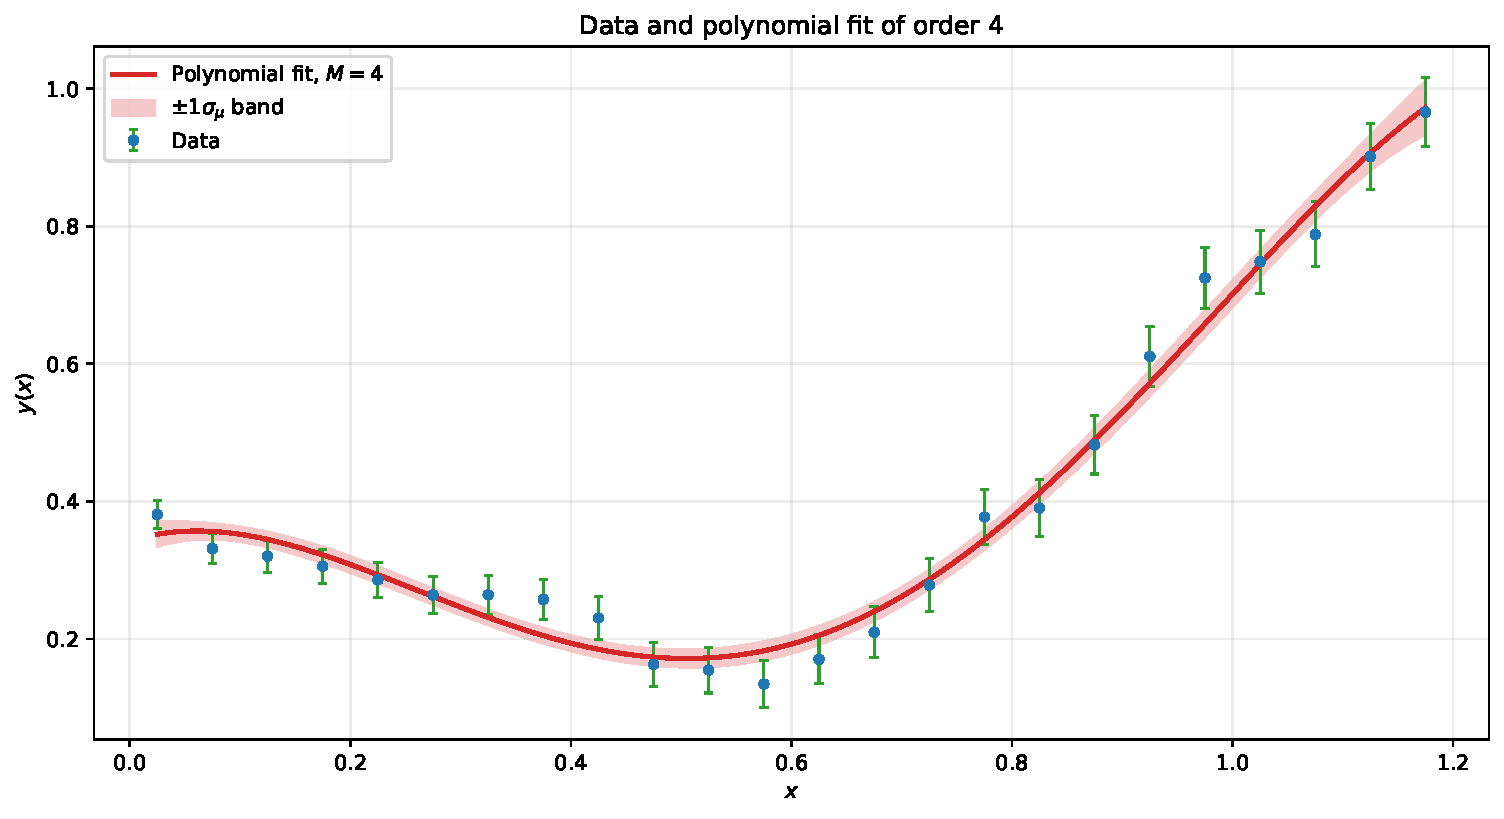
\includegraphics[width=\linewidth]{images/final_fit.pdf}
		\caption{Data and polynomial fit of order $M = 4$, with the band $\mu(x) \pm \sigma_\mu(x)$.}
		\label{fig:final}
	\end{figure}

\end{document}

